\documentclass[12pt,]{article}
\usepackage{lmodern}
\usepackage{amssymb,amsmath}
\usepackage{ifxetex,ifluatex}
\usepackage{fixltx2e} % provides \textsubscript
\ifnum 0\ifxetex 1\fi\ifluatex 1\fi=0 % if pdftex
  \usepackage[T1]{fontenc}
  \usepackage[utf8]{inputenc}
\else % if luatex or xelatex
  \ifxetex
    \usepackage{mathspec}
  \else
    \usepackage{fontspec}
  \fi
  \defaultfontfeatures{Ligatures=TeX,Scale=MatchLowercase}
\fi
% use upquote if available, for straight quotes in verbatim environments
\IfFileExists{upquote.sty}{\usepackage{upquote}}{}
% use microtype if available
\IfFileExists{microtype.sty}{%
\usepackage{microtype}
\UseMicrotypeSet[protrusion]{basicmath} % disable protrusion for tt fonts
}{}
\usepackage[margin=1in]{geometry}
\usepackage{hyperref}
\hypersetup{unicode=true,
            pdftitle={HIV Senegal Model},
            pdfauthor={Fabricia F. Nascimento},
            pdfborder={0 0 0},
            breaklinks=true}
\urlstyle{same}  % don't use monospace font for urls
\usepackage{color}
\usepackage{fancyvrb}
\newcommand{\VerbBar}{|}
\newcommand{\VERB}{\Verb[commandchars=\\\{\}]}
\DefineVerbatimEnvironment{Highlighting}{Verbatim}{commandchars=\\\{\}}
% Add ',fontsize=\small' for more characters per line
\usepackage{framed}
\definecolor{shadecolor}{RGB}{248,248,248}
\newenvironment{Shaded}{\begin{snugshade}}{\end{snugshade}}
\newcommand{\AlertTok}[1]{\textcolor[rgb]{0.94,0.16,0.16}{#1}}
\newcommand{\AnnotationTok}[1]{\textcolor[rgb]{0.56,0.35,0.01}{\textbf{\textit{#1}}}}
\newcommand{\AttributeTok}[1]{\textcolor[rgb]{0.77,0.63,0.00}{#1}}
\newcommand{\BaseNTok}[1]{\textcolor[rgb]{0.00,0.00,0.81}{#1}}
\newcommand{\BuiltInTok}[1]{#1}
\newcommand{\CharTok}[1]{\textcolor[rgb]{0.31,0.60,0.02}{#1}}
\newcommand{\CommentTok}[1]{\textcolor[rgb]{0.56,0.35,0.01}{\textit{#1}}}
\newcommand{\CommentVarTok}[1]{\textcolor[rgb]{0.56,0.35,0.01}{\textbf{\textit{#1}}}}
\newcommand{\ConstantTok}[1]{\textcolor[rgb]{0.00,0.00,0.00}{#1}}
\newcommand{\ControlFlowTok}[1]{\textcolor[rgb]{0.13,0.29,0.53}{\textbf{#1}}}
\newcommand{\DataTypeTok}[1]{\textcolor[rgb]{0.13,0.29,0.53}{#1}}
\newcommand{\DecValTok}[1]{\textcolor[rgb]{0.00,0.00,0.81}{#1}}
\newcommand{\DocumentationTok}[1]{\textcolor[rgb]{0.56,0.35,0.01}{\textbf{\textit{#1}}}}
\newcommand{\ErrorTok}[1]{\textcolor[rgb]{0.64,0.00,0.00}{\textbf{#1}}}
\newcommand{\ExtensionTok}[1]{#1}
\newcommand{\FloatTok}[1]{\textcolor[rgb]{0.00,0.00,0.81}{#1}}
\newcommand{\FunctionTok}[1]{\textcolor[rgb]{0.00,0.00,0.00}{#1}}
\newcommand{\ImportTok}[1]{#1}
\newcommand{\InformationTok}[1]{\textcolor[rgb]{0.56,0.35,0.01}{\textbf{\textit{#1}}}}
\newcommand{\KeywordTok}[1]{\textcolor[rgb]{0.13,0.29,0.53}{\textbf{#1}}}
\newcommand{\NormalTok}[1]{#1}
\newcommand{\OperatorTok}[1]{\textcolor[rgb]{0.81,0.36,0.00}{\textbf{#1}}}
\newcommand{\OtherTok}[1]{\textcolor[rgb]{0.56,0.35,0.01}{#1}}
\newcommand{\PreprocessorTok}[1]{\textcolor[rgb]{0.56,0.35,0.01}{\textit{#1}}}
\newcommand{\RegionMarkerTok}[1]{#1}
\newcommand{\SpecialCharTok}[1]{\textcolor[rgb]{0.00,0.00,0.00}{#1}}
\newcommand{\SpecialStringTok}[1]{\textcolor[rgb]{0.31,0.60,0.02}{#1}}
\newcommand{\StringTok}[1]{\textcolor[rgb]{0.31,0.60,0.02}{#1}}
\newcommand{\VariableTok}[1]{\textcolor[rgb]{0.00,0.00,0.00}{#1}}
\newcommand{\VerbatimStringTok}[1]{\textcolor[rgb]{0.31,0.60,0.02}{#1}}
\newcommand{\WarningTok}[1]{\textcolor[rgb]{0.56,0.35,0.01}{\textbf{\textit{#1}}}}
\usepackage{graphicx,grffile}
\makeatletter
\def\maxwidth{\ifdim\Gin@nat@width>\linewidth\linewidth\else\Gin@nat@width\fi}
\def\maxheight{\ifdim\Gin@nat@height>\textheight\textheight\else\Gin@nat@height\fi}
\makeatother
% Scale images if necessary, so that they will not overflow the page
% margins by default, and it is still possible to overwrite the defaults
% using explicit options in \includegraphics[width, height, ...]{}
\setkeys{Gin}{width=\maxwidth,height=\maxheight,keepaspectratio}
\IfFileExists{parskip.sty}{%
\usepackage{parskip}
}{% else
\setlength{\parindent}{0pt}
\setlength{\parskip}{6pt plus 2pt minus 1pt}
}
\setlength{\emergencystretch}{3em}  % prevent overfull lines
\providecommand{\tightlist}{%
  \setlength{\itemsep}{0pt}\setlength{\parskip}{0pt}}
\setcounter{secnumdepth}{0}
% Redefines (sub)paragraphs to behave more like sections
\ifx\paragraph\undefined\else
\let\oldparagraph\paragraph
\renewcommand{\paragraph}[1]{\oldparagraph{#1}\mbox{}}
\fi
\ifx\subparagraph\undefined\else
\let\oldsubparagraph\subparagraph
\renewcommand{\subparagraph}[1]{\oldsubparagraph{#1}\mbox{}}
\fi

%%% Use protect on footnotes to avoid problems with footnotes in titles
\let\rmarkdownfootnote\footnote%
\def\footnote{\protect\rmarkdownfootnote}

%%% Change title format to be more compact
\usepackage{titling}

% Create subtitle command for use in maketitle
\newcommand{\subtitle}[1]{
  \posttitle{
    \begin{center}\large#1\end{center}
    }
}

\setlength{\droptitle}{-2em}
  \title{HIV Senegal Model}
  \pretitle{\vspace{\droptitle}\centering\huge}
  \posttitle{\par}
  \author{Fabricia F. Nascimento}
  \preauthor{\centering\large\emph}
  \postauthor{\par}
  \predate{\centering\large\emph}
  \postdate{\par}
  \date{2018-05-04}

\usepackage{booktabs}
\usepackage{longtable}
\usepackage{array}
\usepackage{multirow}
\usepackage[table]{xcolor}
\usepackage{wrapfig}
\usepackage{float}
\usepackage{colortbl}
\usepackage{pdflscape}
\usepackage{tabu}
\usepackage{threeparttable}
\usepackage[normalem]{ulem}

\begin{document}
\maketitle

\hypertarget{introduction}{%
\section{Introduction}\label{introduction}}

This vignette will demonstrate how we estimated HIV transmission rates
using DNA sequences from Senegal. This also provides a guidance on how
analysis described in Nascimento \emph{et al}. 2018 (In Prep.) was
carried out. We analysed HIV-1 sequences from subtypes B, C and 02\_AG.

\hypertarget{basic-requirements}{%
\section{Basic requirements}\label{basic-requirements}}

This vignette assumes that you know the basics of R and have the
following packages already installed:

\begin{itemize}
\tightlist
\item
  ape: for phylogenetic trees
\item
  akima: necessary for interpolation of data (used for the calculation
  of the likelihood by the phydynR package)
\item
  \href{\%22https://github.com/florianhartig/BayesianTools\%22}{BayesianTools}:
  package for Bayesian inference
\item
  devtools: useful for installing packages directly from github
  repository, for example.
\item
  \href{\%22https://github.com/emvolz-phylodynamics/phydynR\%22}{phydynR}:
  implements the coalescent simulation and likelihood function for
  phylodynamics analysis
\item
  \href{\%22https://github.com/emvolz/treedater\%22}{treedater}: fits a
  molecular clock to a phylogenetic tree.
\end{itemize}

\hypertarget{load-the-necessary-packages}{%
\subsection{Load the necessary
packages:}\label{load-the-necessary-packages}}

\begin{Shaded}
\begin{Highlighting}[]
  \KeywordTok{library}\NormalTok{(ape)}
  \KeywordTok{library}\NormalTok{(akima)}
  \KeywordTok{library}\NormalTok{(BayesianTools)}
  \KeywordTok{library}\NormalTok{(phydynR)}
  \KeywordTok{library}\NormalTok{(treedater)}
\end{Highlighting}
\end{Shaded}

\hypertarget{the-model}{%
\section{The Model}\label{the-model}}

The model we fit is based on the structured coalescent models (Volz
2012). These models are used to estimate epidemiological parameters
using a phylogenetic tree and information on states of each tip of the
tree. These states are discrete-trait information representing each
sequences.

In our mathematical model we have 4 different discrete-traits associated
to each DNA sequence:

\begin{itemize}
\tightlist
\item
  \(gpf\) = HIV sample from the general population -- females;
\item
  \(gpm\) = HIV sample from the general population -- males;
\item
  \(msm\) = HIV sample from men that have sex with other men;
\item
  \(src\) = source sample, which are HIV samples from individuals that
  are from other countries and not from Senegal.
\end{itemize}

\hypertarget{stage-of-infection}{%
\subsection{Stage of infection}\label{stage-of-infection}}

We fit the HIV epidemic in Senegal using ordinary differential equations
(ODE) and only 1 stage of infection. This means that infected
individuals would die and not recover from the infection. In our model
we represented it as \(\gamma\) rate. We used 1 stage of infection,
because the metadata available for the Senegal sequences did not have
information that we could use to determine the stage of HIV infection at
the time the samples were collected.

\hypertarget{how-transmissions-were-modelled}{%
\subsection{How transmissions were
modelled?}\label{how-transmissions-were-modelled}}

\begin{itemize}
\tightlist
\item
  An infected \(msm\) (\(I_{msm}\)) could transmite to another \(msm\)
  with probability \(p_{msm2msm}\)
\item
  An infected \(msm\) (\(I_{msm}\)) could transmit to a \(gpf\) with
  probability \((1 - p_{msm2msm})\)
\item
  An infected \(gpf\) (\(I_{gpf}\)) could transmit to a \(gpm\) with
  probability \(p_{gpf2gpm}\)
\item
  An infected \(gpf\) (\(I_{gpf}\)) could transmit to a \(msm\) with
  probability \((1 - p_{gpf2gpm})\)
\item
  An infected \(gpm\) could also transmit to a \(gpf\). For this event,
  we used the risk ratio of a male to transmite to a female, and fixed
  it to \(2.0\). This is the parameter \(male_{x}\) of our model.
\end{itemize}

See Figure 1 for a schematic representation of the transmission model
for HIV in Senegal. In this figure \(gpf\), \(gpm\) and \(msm\)
represent the infected individuals.

\begin{figure}

{\centering 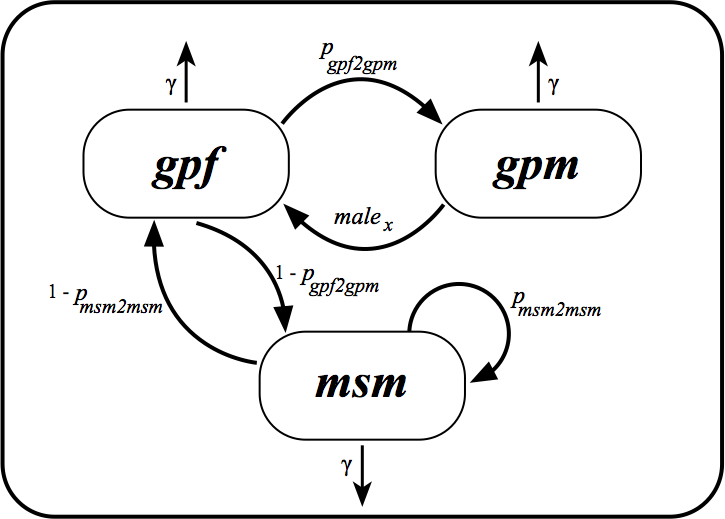
\includegraphics[width=1\linewidth]{images/SN_model_v2} 

}

\caption{Transmission model for HIV in Senegal. $gpf$, $gpm$ and $msm$ represent infected individuals.}\label{fig:unnamed-chunk-2}
\end{figure}

\hypertarget{how-about-hiv-incidence-rate}{%
\subsection{How about HIV incidence
rate?}\label{how-about-hiv-incidence-rate}}

We also modelled the HIV incidence rate as a funtion of time (\(t\)) in
\(msm\) and the \(gp\) (general population) as different spline
functions (Eilers and Marx 1996), that in our ODEs are represented by
\(\lambda(t)\) and \(\mu(t)\), respectively.

\hypertarget{the-source-compartment}{%
\subsection{\texorpdfstring{The \(source\)
compartment}{The source compartment}}\label{the-source-compartment}}

Finally, to model the HIV epidemic in Senegal, we also added an
additional compartment named ``source'' (\(src\)), that represents the
rate in which HIV lineages are imported to Senegal from other countries.
We modelled this as a constant efective population size rate with two
parameters to be estimeted -- \(srcNe\): the effective source population
size; and the \(import\) rate. Because the number of imported HIV
balances the number of exported HIV, the infected \(src\) individuals
along time are not represented in the ODEs.

\hypertarget{the-odes-or-mathematical-model-equations}{%
\subsection{The ODEs or mathematical model
equations}\label{the-odes-or-mathematical-model-equations}}

Based on \textbf{Figure 1} and the parameters we would like to estimate,
the ordinary differential equations (ODEs) of our model are:

\(\dot{I}_{gpf} = male_x \mu(t) I_{gpm} + (1 - p_{msm2msm}) \lambda(t) I_{msm} - \gamma I_{gpf}\)

\(\dot{I}_{gpm} = p_{gpf2gpm} \mu(t) I_{gpf} - \gamma I_{gpm}\)

\(\dot{I}_{msm} = (1 - p_{gpf2gpm}) \mu(t) I_{gpf} + p_{msm2msm} \lambda(t) I_{msm} - \gamma I_{msm}\)

\hypertarget{how-to-express-the-mathematical-model-in-r}{%
\subsection{How to express the mathematical model in
R?}\label{how-to-express-the-mathematical-model-in-r}}

In our model, we are interested in HIV transmissions in the \(gp\) and
in the \(msm\) risk group. But also remember that we have to consider
the imported HIV, which is in the \(src\) compartment. Based on that,
\(gpf\), \(gpm\), \(msm\), and \(src\) are the demes of our model, and
are represented as a vector in R as:

\begin{Shaded}
\begin{Highlighting}[]
\NormalTok{demes <-}\StringTok{ }\KeywordTok{c}\NormalTok{(}\StringTok{"gpm"}\NormalTok{, }\StringTok{"gpf"}\NormalTok{, }\StringTok{"msm"}\NormalTok{, }\StringTok{"src"}\NormalTok{)}
\end{Highlighting}
\end{Shaded}

Because we use spline functions to determine the shape of the curve for
the transmission rates in \(gp\) and \(msm\), we should provide the
initial \texttt{T0} and final \texttt{T1} times for our simulations.

\begin{Shaded}
\begin{Highlighting}[]
\NormalTok{T0 <-}\StringTok{ }\DecValTok{1978}
\NormalTok{T1 <-}\StringTok{ }\DecValTok{2014}
\end{Highlighting}
\end{Shaded}

We can also go ahead and set the value for the stage of infection, that
in our model is just one stage. We assume we know this value.

\begin{Shaded}
\begin{Highlighting}[]
\NormalTok{GAMMA <-}\StringTok{ }\DecValTok{1}\OperatorTok{/}\DecValTok{10}
\end{Highlighting}
\end{Shaded}

We should also create a list to set up a template for the parameter
values of our model. You can set this to values that you think are
appropriate. Remember that the majority of parameter values in this list
will be estimated. In R, this can be created following:

\begin{Shaded}
\begin{Highlighting}[]
\NormalTok{THETA <-}\StringTok{ }\KeywordTok{list}\NormalTok{(}\DataTypeTok{gpsp0 =} \DecValTok{6}\OperatorTok{/}\DecValTok{10}\NormalTok{,}
              \DataTypeTok{gpsp1 =} \DecValTok{4}\OperatorTok{/}\DecValTok{10}\NormalTok{,}
              \DataTypeTok{gpsp2 =} \DecValTok{1}\OperatorTok{/}\DecValTok{10}\NormalTok{,}
              \DataTypeTok{gpsploc =} \DecValTok{1987}\NormalTok{,}
              \DataTypeTok{msmsp0 =} \DecValTok{4}\OperatorTok{/}\DecValTok{10}\NormalTok{,}
              \DataTypeTok{msmsp1 =} \DecValTok{4}\OperatorTok{/}\DecValTok{10}\NormalTok{,}
              \DataTypeTok{msmsp2 =} \DecValTok{2}\OperatorTok{/}\DecValTok{10}\NormalTok{,}
              \DataTypeTok{msmsploc =} \DecValTok{1995}\NormalTok{,}
              \DataTypeTok{maleX =} \FloatTok{2.0}\NormalTok{,}
              \DataTypeTok{import =} \DecValTok{1}\OperatorTok{/}\DecValTok{20}\NormalTok{,}
              \DataTypeTok{srcNe =} \DecValTok{1}\OperatorTok{/}\DecValTok{10}\NormalTok{,}
              \DataTypeTok{gpspline =} \ControlFlowTok{function}\NormalTok{(t, parms)\{}
                \ControlFlowTok{if}\NormalTok{ (t }\OperatorTok{<}\StringTok{ }\NormalTok{T0) }\KeywordTok{return}\NormalTok{(parms}\OperatorTok{$}\NormalTok{gpsp0)}
                \ControlFlowTok{if}\NormalTok{ (t }\OperatorTok{>}\StringTok{ }\NormalTok{T1) }\KeywordTok{return}\NormalTok{ (parms}\OperatorTok{$}\NormalTok{gpsp2)}
                \KeywordTok{with}\NormalTok{(parms, }\KeywordTok{aspline}\NormalTok{(}\DataTypeTok{x =} \KeywordTok{c}\NormalTok{(T0, gpsploc, T1), }
                                    \DataTypeTok{y=}\KeywordTok{c}\NormalTok{(gpsp0, gpsp1, gpsp2), }
                                    \DataTypeTok{xout =}\NormalTok{ t)}\OperatorTok{$}\NormalTok{y)}
\NormalTok{              \},}
              \DataTypeTok{msmspline  =} \ControlFlowTok{function}\NormalTok{(t, parms)\{}
                \ControlFlowTok{if}\NormalTok{ (t }\OperatorTok{<}\StringTok{ }\NormalTok{T0) }\KeywordTok{return}\NormalTok{(parms}\OperatorTok{$}\NormalTok{msmsp0)}
                \ControlFlowTok{if}\NormalTok{ (t }\OperatorTok{>}\StringTok{ }\NormalTok{T1) }\KeywordTok{return}\NormalTok{ (parms}\OperatorTok{$}\NormalTok{msmsp2)}
                \KeywordTok{with}\NormalTok{(parms, }\KeywordTok{aspline}\NormalTok{(}\DataTypeTok{x =} \KeywordTok{c}\NormalTok{(T0, msmsploc, T1), }
                                    \DataTypeTok{y=}\KeywordTok{c}\NormalTok{(msmsp0, msmsp1, msmsp2), }
                                    \DataTypeTok{xout =}\NormalTok{ t)}\OperatorTok{$}\NormalTok{y)}
\NormalTok{              \},}
             \DataTypeTok{pmsm2msm =} \FloatTok{0.85}\NormalTok{,}
             \DataTypeTok{pgpf2gpm =} \FloatTok{0.85}\NormalTok{,}
             \DataTypeTok{initmsm =} \DecValTok{1}\NormalTok{,}
             \DataTypeTok{initgp =} \DecValTok{1}\NormalTok{)}
\end{Highlighting}
\end{Shaded}

Note that parameters \(gpsp0\), \(gpsp1\), \(gpsp2\), and \(gpsploc\)
are necessary to estimate the spline function for the \(gp\)
(\(gpspline\) in R or \(\mu(t)\) in the ODE). And parameters \(msmsp0\),
\(msmsp1\), \(msmsp2\), \(msmsploc\) are necessary to estimate the
spline function for the \(msm\) risk group (\(msmspline\) in R or
\(\lambda(t)\) in the ODE).

\rowcolors{2}{gray!6}{white}
\begin{table}

\caption{\label{tab:unnamed-chunk-7}Parameter definition, values and symbols used in the R script}
\centering
\begin{tabular}[t]{lll}
\hiderowcolors
\toprule
Parameter & Symbol in R & Initial values\\
\midrule
\showrowcolors
Spline shape gp0 & gpsp0 & 6/10\\
Spline shape gp1 & gpsp1 & 4/10\\
Spline shape gp2 & gpsp2 & 1/10\\
Spline interval gp & gpsploc & 1987\\
Spline shape msm0 & msmsp0 & 4/10\\
\addlinespace
Spline shape msm1 & msmsp1 & 4/10\\
Spline shape msm2 & msmsp2 & 2/10\\
Spline interval msm & msmsploc & 1995\\
Infectiouness ratio from male to female & maleX & 2.0\\
Importation rate & import & 1.20\\
\addlinespace
Effective population size of src & srcNe & 1.10\\
Probability of infected msm to infect another msm & pmsm2msm & 0.85\\
Probability of infected gpf to infect a gpm & pgpf2gpm & 0.85\\
Initial number of infected msm & initmsm & 1.0\\
Initial number of infected gp & initgp & 1.0\\
\bottomrule
\end{tabular}
\end{table}
\rowcolors{2}{white}{white}

We also need to setup some initial conditions of our model. We should
set an arbitrary large number for the \(src\) population,

\begin{Shaded}
\begin{Highlighting}[]
\NormalTok{SRCSIZE <<-}\StringTok{ }\FloatTok{1e5}
\NormalTok{X0 <-}\StringTok{ }\KeywordTok{c}\NormalTok{(}\DataTypeTok{gpm =} \KeywordTok{unname}\NormalTok{(THETA}\OperatorTok{$}\NormalTok{initgp}\OperatorTok{/}\DecValTok{2}\NormalTok{),}
        \DataTypeTok{gpf =} \KeywordTok{unname}\NormalTok{(THETA}\OperatorTok{$}\NormalTok{initgp}\OperatorTok{/}\DecValTok{2}\NormalTok{),}
        \DataTypeTok{msm =} \KeywordTok{unname}\NormalTok{(THETA}\OperatorTok{$}\NormalTok{initmsm),}
        \DataTypeTok{src =}\NormalTok{ SRCSIZE)}
\end{Highlighting}
\end{Shaded}

\hypertarget{setting-up-the-birth-migration-and-death-rates}{%
\subsubsection{Setting up the birth, migration and death
rates}\label{setting-up-the-birth-migration-and-death-rates}}

The calculation of births and migrations of our model are expressed as 4
\(\times\) 4 matrices, which represent a transmission or movement from
one deme to another deme. Lineages also die at a same rate.

First, we have to setup the components of the model. This can be done
using the \texttt{setup.model.equations} function in this research
compendium.

\begin{Shaded}
\begin{Highlighting}[]
\NormalTok{eqns <-}\StringTok{ }\NormalTok{senegalHIVmodel}\OperatorTok{::}\KeywordTok{setup.model.equations}\NormalTok{(demes)}
\KeywordTok{attach}\NormalTok{(eqns)}
\end{Highlighting}
\end{Shaded}

\hypertarget{setting-up-the-birth-matrix}{%
\subsubsection{Setting up the birth
matrix}\label{setting-up-the-birth-matrix}}

We should set up the birth matrix to allow transmissions from one deme
to another deme as in \textbf{Figure 1}.

\rowcolors{2}{gray!6}{white}
\begin{table}

\caption{\label{tab:unnamed-chunk-10}Illustration of allowed transmissions between demes.}
\centering
\begin{tabular}[t]{>{\bfseries}lllll}
\hiderowcolors
\toprule
  & gpm & gpf & msm & src\\
\midrule
\showrowcolors
gpm & 0. & $gpm \to gpf$ & 0. & 0.\\
gpf & $gpf \to gpm$ & 0. & $gpf \to msm$ & 0.\\
msm & 0. & $msm \to gpf$ & $msm \to msm$ & 0.\\
src & 0. & 0. & 0. & $src \to src$\\
\bottomrule
\end{tabular}
\end{table}
\rowcolors{2}{white}{white}

To set up these transmissions between demes, each element in the matrix
is a string that will be passed as R code.

\begin{Shaded}
\begin{Highlighting}[]
\NormalTok{births[}\StringTok{'msm'}\NormalTok{, }\StringTok{'msm'}\NormalTok{] <-}\StringTok{ "parms$msmspline(t, parms) * msm * parms$pmsm2msm"}
\NormalTok{births[}\StringTok{'msm'}\NormalTok{, }\StringTok{'gpf'}\NormalTok{] <-}\StringTok{ "parms$msmspline(t, parms) * msm * (1-parms$pmsm2msm)"}

\NormalTok{births[}\StringTok{'gpm'}\NormalTok{, }\StringTok{'gpf'}\NormalTok{] <-}\StringTok{ "parms$gpspline(t, parms) * gpm * parms$maleX"}
\NormalTok{births[}\StringTok{'gpf'}\NormalTok{, }\StringTok{'gpm'}\NormalTok{] <-}\StringTok{ "parms$gpspline(t, parms) * gpf * parms$pgpf2gpm"}
\NormalTok{births[}\StringTok{'gpf'}\NormalTok{, }\StringTok{'msm'}\NormalTok{] <-}\StringTok{ "parms$gpspline(t, parms) * gpf * (1-parms$pgpf2gpm)"}

\CommentTok{# f = (1/2)*(Y^2)/Ne}
\NormalTok{births[}\StringTok{'src'}\NormalTok{, }\StringTok{'src'}\NormalTok{] <-}\StringTok{ "0.5 * SRCSIZE^2 / parms$srcNe"}
\end{Highlighting}
\end{Shaded}

\hypertarget{setting-up-the-migration-matrix}{%
\subsubsection{Setting up the migration
matrix}\label{setting-up-the-migration-matrix}}

Similar to the birth matrix, we also allow migrations from \(gpf\),
\(gpm\), or \(msm\) to the \(src\); and from \(src\) to \(gpf\),
\(gpm\), or \(msm\). This is modelled as a constant effective population
size.

\rowcolors{2}{gray!6}{white}
\begin{table}[!h]

\caption{\label{tab:unnamed-chunk-12}Illustration of allowed migrations between demes.}
\centering
\begin{tabular}[t]{>{\bfseries}lllll}
\hiderowcolors
\toprule
  & gpm & gpf & msm & src\\
\midrule
\showrowcolors
gpm & 0. & 0. & 0. & $gpm \to src$\\
gpf & 0. & 0. & 0. & $gpf \to src$\\
msm & 0. & 0. & 0. & $msm \to src$\\
src & $src \to gpm$ & $src \to gpf$ & $src \to msm$ & 0.\\
\bottomrule
\end{tabular}
\end{table}
\rowcolors{2}{white}{white}

We also set up migrations between demes where each element in the matrix
is a string that will be passed as R code.

\begin{Shaded}
\begin{Highlighting}[]
\NormalTok{migs[}\StringTok{'src'}\NormalTok{, }\StringTok{'gpm'}\NormalTok{] <-}\StringTok{ "parms$import * gpm"}
\NormalTok{migs[}\StringTok{'src'}\NormalTok{, }\StringTok{'gpf'}\NormalTok{] <-}\StringTok{ "parms$import * gpf"}
\NormalTok{migs[}\StringTok{'src'}\NormalTok{, }\StringTok{'msm'}\NormalTok{] <-}\StringTok{ "parms$import * msm"}

\NormalTok{migs[}\StringTok{'gpm'}\NormalTok{, }\StringTok{'src'}\NormalTok{] <-}\StringTok{ "parms$import * gpm"}
\NormalTok{migs[}\StringTok{'gpf'}\NormalTok{, }\StringTok{'src'}\NormalTok{] <-}\StringTok{ "parms$import * gpf"}
\NormalTok{migs[}\StringTok{'msm'}\NormalTok{, }\StringTok{'src'}\NormalTok{] <-}\StringTok{ "parms$import * msm"}
\end{Highlighting}
\end{Shaded}

\hypertarget{setting-up-the-vector-for-the-death-rates}{%
\subsubsection{Setting up the vector for the death
rates}\label{setting-up-the-vector-for-the-death-rates}}

Similarly to the birth and migration matrices, we also set up death
rates where each element is a string that will be passed as R code.

\begin{Shaded}
\begin{Highlighting}[]
\NormalTok{deaths[}\StringTok{'msm'}\NormalTok{] <-}\StringTok{ "GAMMA * msm"}
\NormalTok{deaths[}\StringTok{'gpf'}\NormalTok{] <-}\StringTok{ "GAMMA * gpf"}
\NormalTok{deaths[}\StringTok{'gpm'}\NormalTok{] <-}\StringTok{ "GAMMA * gpm"}
\NormalTok{deaths[}\StringTok{'src'}\NormalTok{] <-}\StringTok{ "0.5 * SRCSIZE^2 / parms$srcNe"}
\end{Highlighting}
\end{Shaded}

\hypertarget{the-demographic-model}{%
\subsubsection{The demographic model}\label{the-demographic-model}}

After setting up all the components of the mathematical model, we can
build the demographic process using the function
\texttt{build.demographic.process} from the \texttt{phydynR} pachage.
The \texttt{dm} output can be used as imput to coalescent models for the
calculation of the likelihood, when fitting the model using a Markov
chain Monte Carlo (MCMC), for example.

\begin{Shaded}
\begin{Highlighting}[]
\NormalTok{dm <-}\StringTok{ }\KeywordTok{build.demographic.process}\NormalTok{(}\DataTypeTok{births =}\NormalTok{ births,}
                                \DataTypeTok{deaths =}\NormalTok{ deaths,}
                                \DataTypeTok{migrations =}\NormalTok{ migs,}
                                \DataTypeTok{parameterNames =} \KeywordTok{names}\NormalTok{(THETA),}
                                \DataTypeTok{rcpp =} \OtherTok{FALSE}\NormalTok{,}
                                \DataTypeTok{sde =} \OtherTok{FALSE}\NormalTok{)}
\end{Highlighting}
\end{Shaded}

For more information on the the input data for the
\texttt{build.demographic.process} funtion, you should see its R
documentaion.

\hypertarget{load-additional-data}{%
\subsection{Load additional data}\label{load-additional-data}}

After setting up all the equations of the model in a way that R can
understand, the model can now be fitted to a binary and dated
phylogenetic tree. In our specific case, we estimated a phylogenetic
tree using \href{https://github.com/amkozlov/raxml-ng}{RAxML-NG} for
each subtype, as we are analysing HIV-1 subtypes B, C and 02\_AG.

Each tree had a relaxed clock fitted using the R package
\href{https://github.com/emvolz/treedater}{treedater}. And after that,
the trees were merged into a single tree using the R script
\emph{merge\_trees.R} (it can be found in the directory
\texttt{analysis/scripts}). The final tree did not contain sequences
from children, and from which risk group or sex was NA.

We load the binary dated tree in R using the following:

\begin{Shaded}
\begin{Highlighting}[]
\NormalTok{tree.all <-}\StringTok{ }\KeywordTok{read.tree}\NormalTok{(}
  \KeywordTok{system.file}\NormalTok{(}\StringTok{"data/bindTree_CGR_GTR+Gp12+3_droppedTip.tre"}\NormalTok{, }
  \DataTypeTok{package =} \StringTok{"senegalHIVmodel"}\NormalTok{))}
\end{Highlighting}
\end{Shaded}

After, we should load all the information for the metadata. This aims to
create a discrete-trait data for all tips in the phylogenetic tree.
Remember that our discrete-trait data in this model are the \emph{gpf},
\emph{gpm}, \emph{msm}, and \emph{src}.

First we need to read in R all metadata as below:

\begin{Shaded}
\begin{Highlighting}[]
\CommentTok{# Reads metadata for the CGR (close global reference) sequences}
\CommentTok{# CGRs are referred in the mathematical model as src (source) data}
\CommentTok{# src are HIV sequences that are from other countries and not from Senegal}
\NormalTok{all.data.cgr <-}\StringTok{ }\KeywordTok{read.csv}\NormalTok{(}
  \KeywordTok{system.file}\NormalTok{(}\StringTok{"data/HIV_subtypes_summary_CGR.csv"}\NormalTok{, }
  \DataTypeTok{package =} \StringTok{"senegalHIVmodel"}\NormalTok{))}

\CommentTok{# Reads all metadata for HIV sequences from Senegal}
\NormalTok{all.data.SN <-}\StringTok{ }\KeywordTok{read.csv}\NormalTok{(}
  \KeywordTok{system.file}\NormalTok{(}\StringTok{"data/HIV_subtypes_summary_SENEGAL_noDups.csv"}\NormalTok{, }
  \DataTypeTok{package =} \StringTok{"senegalHIVmodel"}\NormalTok{))}

\CommentTok{# organize metadata in 2 columns.}
\CommentTok{# the 1st column is the sequence names}
\CommentTok{# the 2nd colum is the state (gpf, gpm, msm, or src) of each sequence}
\CommentTok{# metadata from children, or risk group or sex = NA will also be removed. }
\NormalTok{all_data <-}\StringTok{ }\NormalTok{senegalHIVmodel}\OperatorTok{::}\KeywordTok{organize_metadata}\NormalTok{(all.data.cgr, all.data.SN)}
\end{Highlighting}
\end{Shaded}

After organing all metadata, we further organize it in a way that the R
package \texttt{phydynR} will understand it. For that, we create a
matrix to receive the information on states (discrete-traits) for each
tip of the tree

\begin{Shaded}
\begin{Highlighting}[]
\NormalTok{gpm <-}\StringTok{ }\NormalTok{gpf <-}\StringTok{ }\NormalTok{msm <-}\StringTok{ }\NormalTok{src <-}\StringTok{ }\KeywordTok{rep}\NormalTok{(}\DecValTok{0}\NormalTok{, }\KeywordTok{length}\NormalTok{(tree.all}\OperatorTok{$}\NormalTok{tip.label))}

\CommentTok{# Adds 1 to where states matches "gpm", and so on.}
\NormalTok{gpm[all_data}\OperatorTok{$}\NormalTok{States }\OperatorTok{==}\StringTok{ "gpm"}\NormalTok{] <-}\StringTok{ }\DecValTok{1}
\NormalTok{gpf[all_data}\OperatorTok{$}\NormalTok{States }\OperatorTok{==}\StringTok{ "gpf"}\NormalTok{] <-}\StringTok{ }\DecValTok{1}
\NormalTok{msm[all_data}\OperatorTok{$}\NormalTok{States }\OperatorTok{==}\StringTok{ "msm"}\NormalTok{] <-}\StringTok{ }\DecValTok{1}
\NormalTok{src[all_data}\OperatorTok{$}\NormalTok{States }\OperatorTok{==}\StringTok{ "src"}\NormalTok{] <-}\StringTok{ }\DecValTok{1}

\NormalTok{sampleStates <-}\StringTok{ }\KeywordTok{cbind}\NormalTok{(gpm, gpf, msm, src)}
\KeywordTok{rownames}\NormalTok{(sampleStates) <-}\StringTok{ }\NormalTok{all_data}\OperatorTok{$}\NormalTok{tip.name}
\end{Highlighting}
\end{Shaded}

Now, we need to read the estimated times (in calendar units) for each
sequence in the phylogenetic tree

\begin{Shaded}
\begin{Highlighting}[]
\NormalTok{times <-}\StringTok{ }\KeywordTok{readRDS}\NormalTok{(}
  \KeywordTok{system.file}\NormalTok{(}\StringTok{"data/bindTree_CGR_GTR+Gp12+3_droppedTip_sts.RDS"}\NormalTok{,}
  \DataTypeTok{package =} \StringTok{"senegalHIVmodel"}\NormalTok{))}
\end{Highlighting}
\end{Shaded}

Finaly, we create an an object of \texttt{DatedTree} {[}phydynR
package{]}. This is the tree that should be used in the calculation of
the likelihood to estimate parameter values using \texttt{phydynR}

\begin{Shaded}
\begin{Highlighting}[]
\NormalTok{dated.tree <-}\StringTok{ }\NormalTok{phydynR}\OperatorTok{::}\KeywordTok{DatedTree}\NormalTok{(}\DataTypeTok{phylo =}\NormalTok{ tree.all,}
                                 \DataTypeTok{sampleTimes =}\NormalTok{ times,}
                                 \DataTypeTok{sampleStates =}\NormalTok{ sampleStates,}
                                 \DataTypeTok{minEdgeLength =} \DecValTok{2}\OperatorTok{/}\DecValTok{52}\NormalTok{,}
                                 \DataTypeTok{tol =} \FloatTok{0.1}\NormalTok{)}
\end{Highlighting}
\end{Shaded}

\hypertarget{calculation-of-the-likelihood}{%
\section{Calculation of the
likelihood}\label{calculation-of-the-likelihood}}

After setting up the mathematical model and the data, we have the
following:

\begin{itemize}
\tightlist
\item
  \texttt{dated.tree} = a phylogenetic tree of class DatedTree
\item
  \texttt{THETA} = template for parameter values
\item
  \texttt{dm} = the demographic process
\item
  \texttt{X0} = initial conditions
\end{itemize}

The above objects will be used in the calculation of the likelihoood
using the \texttt{colik} function in the phydynR package.

\begin{Shaded}
\begin{Highlighting}[]
\NormalTok{phydynR}\OperatorTok{::}\KeywordTok{colik}\NormalTok{(}\DataTypeTok{tree =}\NormalTok{ dated.tree,}
               \DataTypeTok{theta =}\NormalTok{ THETA,}
               \DataTypeTok{demographic.process.model =}\NormalTok{ dm,}
               \DataTypeTok{x0 =}\NormalTok{ X0,}
               \DataTypeTok{t0 =} \DecValTok{1978}\NormalTok{,}
               \DataTypeTok{res =} \FloatTok{1e3}\NormalTok{,}
               \DataTypeTok{timeOfOriginBoundaryCondition =} \OtherTok{FALSE}\NormalTok{,}
               \DataTypeTok{AgtY_penalty =} \DecValTok{1}\NormalTok{,}
               \DataTypeTok{maxHeight =} \DecValTok{41}\NormalTok{)}
\end{Highlighting}
\end{Shaded}

Note that for the calculation of the likelihood you can provide a value
for maximum height \texttt{maxHeight}. This parameter ``tells'' the
function up to which point back in time the calculation of the
likelihood should be done. If computer resources are not a problem, you
can leave this as the default. Using the whole tree for the calculation
of the likelihood can make it slower than when using just a portion back
in time.

For the Senegal data, we used a \texttt{maxHeight} = 41. This means that
it will go back in time in the tree at approximatelly 1973. This was
merely chosen to put the HIV epidemics in Senegal around this time, for
estimation of the parameters in our model.

\hypertarget{estimation-of-epidemiological-parameters}{%
\section{Estimation of epidemiological
parameters}\label{estimation-of-epidemiological-parameters}}

Now that we are happy with everything, we are ready to estimate the
parameters of our model. For the Senegal HIV model, we chose to estimate
the parameters using a Markov chain Monte Carlo (MCMC) as implemented in
the R package
\href{\%22https://github.com/florianhartig/BayesianTools\%22}{BayesianTools}.

\hypertarget{which-parameters-to-estimate}{%
\subsection{Which parameters to
estimate?}\label{which-parameters-to-estimate}}

For this example, we decided to estimate the following parameters:

\textbf{Paramters for estimating the spline function for the \emph{gp}:}

\begin{itemize}
\tightlist
\item
  \emph{gpsp0}
\item
  \emph{gpsp1}
\item
  \emph{gpsp2}
\item
  \emph{gpsploc}
\end{itemize}

\textbf{Parameters for estimating the spline function for the
\emph{msm}:}

\begin{itemize}
\tightlist
\item
  \emph{msmsp0}
\item
  \emph{msmsp1}
\item
  \emph{msmsp2}
\item
  \emph{msmsploc}
\end{itemize}

\textbf{Parameters that controls the \emph{src}:}

\begin{itemize}
\tightlist
\item
  \emph{import}
\item
  \emph{srcNe}
\end{itemize}

\textbf{Probability of certain events to occour:}

\begin{itemize}
\tightlist
\item
  \emph{pmsm2msm}
\item
  \emph{pgpf2gpm}
\end{itemize}

To estimate these parameters we should set up an object function. This
object function will receive the proposals of the MCMC. The reason of
using an object function is to make it easier to change the values of
the parameters to be estimated in THETA (our parameter template as
explained before). Note that not all parameters listed in THETA will be
estimated.

\begin{Shaded}
\begin{Highlighting}[]
\NormalTok{obj_fun <-}\StringTok{ }\ControlFlowTok{function}\NormalTok{(parameters)\{}
  \CommentTok{# we use unname here because "parameters" can be a vector or matrix, and}
  \CommentTok{# sometimes it comes with column names, which I chose to remove these names}
  \CommentTok{# in here.}
\NormalTok{  parameters <-}\StringTok{ }\KeywordTok{unname}\NormalTok{(parameters)}

  \CommentTok{# add the values of THETA to a new variable named THETA.new}
\NormalTok{  THETA.new <-}\StringTok{ }\NormalTok{THETA}

  \CommentTok{# change the values in THETA.new to the new proposals that will be evaluated}
\NormalTok{  THETA.new}\OperatorTok{$}\NormalTok{gpsp0 <-}\StringTok{ }\NormalTok{parameters[}\DecValTok{1}\NormalTok{]}
\NormalTok{  THETA.new}\OperatorTok{$}\NormalTok{gpsp1 <-}\StringTok{ }\NormalTok{parameters[}\DecValTok{2}\NormalTok{]}
\NormalTok{  THETA.new}\OperatorTok{$}\NormalTok{gpsp2 <-}\StringTok{ }\NormalTok{parameters[}\DecValTok{3}\NormalTok{]}
\NormalTok{  THETA.new}\OperatorTok{$}\NormalTok{gpsploc <-}\StringTok{ }\NormalTok{parameters[}\DecValTok{4}\NormalTok{]}
\NormalTok{  THETA.new}\OperatorTok{$}\NormalTok{msmsp0 <-}\StringTok{ }\NormalTok{parameters[}\DecValTok{5}\NormalTok{]}
\NormalTok{  THETA.new}\OperatorTok{$}\NormalTok{msmsp1 <-}\StringTok{ }\NormalTok{parameters[}\DecValTok{6}\NormalTok{]}
\NormalTok{  THETA.new}\OperatorTok{$}\NormalTok{msmsp2 <-}\StringTok{ }\NormalTok{parameters[}\DecValTok{7}\NormalTok{]}
\NormalTok{  THETA.new}\OperatorTok{$}\NormalTok{msmsploc <-}\StringTok{ }\NormalTok{parameters[}\DecValTok{8}\NormalTok{]}
\NormalTok{  THETA.new}\OperatorTok{$}\NormalTok{import <-}\StringTok{ }\NormalTok{parameters[}\DecValTok{9}\NormalTok{]}
\NormalTok{  THETA.new}\OperatorTok{$}\NormalTok{srcNe <-}\StringTok{ }\NormalTok{parameters[}\DecValTok{10}\NormalTok{]}
\NormalTok{  THETA.new}\OperatorTok{$}\NormalTok{pmsm2msm <-}\StringTok{ }\NormalTok{parameters[}\DecValTok{11}\NormalTok{]}
\NormalTok{  THETA.new}\OperatorTok{$}\NormalTok{pgpf2gpm <-}\StringTok{ }\NormalTok{parameters[}\DecValTok{12}\NormalTok{]}

  \CommentTok{# After changing the parameter values to the new proposals, a likelihood is}
  \CommentTok{# calculated with the funtion colik.}
  \CommentTok{# Note that this function uses several global variables, such as, }
  \CommentTok{# dated.tree, dm, and X0}
\NormalTok{  mll <-}\StringTok{ }\NormalTok{phydyn}\OperatorTok{::}\KeywordTok{colik}\NormalTok{(}\DataTypeTok{tree =}\NormalTok{ dated.tree,}
               \DataTypeTok{theta =}\NormalTok{ THETA.new,}
               \DataTypeTok{demographic.process.model =}\NormalTok{ dm,}
               \DataTypeTok{x0 =}\NormalTok{ X0,}
               \DataTypeTok{t0 =} \DecValTok{1978}\NormalTok{,}
               \DataTypeTok{res =} \FloatTok{1e3}\NormalTok{,}
               \DataTypeTok{timeOfOriginBoundaryCondition =} \OtherTok{FALSE}\NormalTok{,}
               \DataTypeTok{AgtY_penalty =} \DecValTok{1}\NormalTok{,}
               \DataTypeTok{maxHeight =} \DecValTok{41}\NormalTok{)}

  \KeywordTok{return}\NormalTok{(mll)}

\NormalTok{\}}
\end{Highlighting}
\end{Shaded}

We can now estimate these parameters using the MCMC. For that we need to
decide the priors -- our best knowledge on the parameter value before
the data is analysed -- on each parameter that will be estimated.

Because we are using the BayesianTools R package, we need to specify the
density function (that represent our prior) for each parameter as below:

\begin{Shaded}
\begin{Highlighting}[]
\CommentTok{# Specify a density function to be used in the }
\CommentTok{# prior especification (see below)}
\NormalTok{densities <-}\StringTok{  }\ControlFlowTok{function}\NormalTok{(par)\{}
  \CommentTok{# d1 to d3 and d5 to d7 I am using a gamma distribution with }
  \CommentTok{#    mean = R0 = 1.1 and sigma = 1}
  \CommentTok{# d4, d8 uniform distribution between the start time and }
  \CommentTok{# the final time of our simualtions (t0 = 1978, and t1 = 2014)}
  \CommentTok{# d9 exponential distribution with mean around 1/30}
  \CommentTok{# d10 exponential distribution with mean around 1/20}
\NormalTok{  d1 =}\StringTok{ }\KeywordTok{dgamma}\NormalTok{(par[}\DecValTok{1}\NormalTok{], }\DataTypeTok{shape =} \DecValTok{3}\NormalTok{, }\DataTypeTok{rate =} \DecValTok{3}\OperatorTok{/}\FloatTok{1.1}\NormalTok{, }\DataTypeTok{log =} \OtherTok{TRUE}\NormalTok{) }\CommentTok{#gpsp0}
\NormalTok{  d2 =}\StringTok{ }\KeywordTok{dgamma}\NormalTok{(par[}\DecValTok{2}\NormalTok{], }\DataTypeTok{shape =} \DecValTok{3}\NormalTok{, }\DataTypeTok{rate =} \DecValTok{3}\OperatorTok{/}\FloatTok{1.1}\NormalTok{, }\DataTypeTok{log =} \OtherTok{TRUE}\NormalTok{) }\CommentTok{#gpsp1}
\NormalTok{  d3 =}\StringTok{ }\KeywordTok{dgamma}\NormalTok{(par[}\DecValTok{3}\NormalTok{], }\DataTypeTok{shape =} \DecValTok{3}\NormalTok{, }\DataTypeTok{rate =} \DecValTok{3}\OperatorTok{/}\FloatTok{1.1}\NormalTok{, }\DataTypeTok{log =} \OtherTok{TRUE}\NormalTok{) }\CommentTok{#gpsp2}
\NormalTok{  d4 =}\StringTok{ }\KeywordTok{dunif}\NormalTok{(par[}\DecValTok{4}\NormalTok{], }\DataTypeTok{min =} \DecValTok{1978}\NormalTok{, }\DataTypeTok{max =} \DecValTok{2014}\NormalTok{, }\DataTypeTok{log =} \OtherTok{TRUE}\NormalTok{) }\CommentTok{#gpsploc}
\NormalTok{  d5 =}\StringTok{ }\KeywordTok{dgamma}\NormalTok{(par[}\DecValTok{5}\NormalTok{], }\DataTypeTok{shape =} \DecValTok{3}\NormalTok{, }\DataTypeTok{rate =} \DecValTok{3}\OperatorTok{/}\FloatTok{1.1}\NormalTok{, }\DataTypeTok{log =} \OtherTok{TRUE}\NormalTok{) }\CommentTok{#msmsp0}
\NormalTok{  d6 =}\StringTok{ }\KeywordTok{dgamma}\NormalTok{(par[}\DecValTok{6}\NormalTok{], }\DataTypeTok{shape =} \DecValTok{3}\NormalTok{, }\DataTypeTok{rate =} \DecValTok{3}\OperatorTok{/}\FloatTok{1.1}\NormalTok{, }\DataTypeTok{log =} \OtherTok{TRUE}\NormalTok{) }\CommentTok{#msmsp1}
\NormalTok{  d7 =}\StringTok{ }\KeywordTok{dgamma}\NormalTok{(par[}\DecValTok{7}\NormalTok{], }\DataTypeTok{shape =} \DecValTok{3}\NormalTok{, }\DataTypeTok{rate =} \DecValTok{3}\OperatorTok{/}\FloatTok{1.1}\NormalTok{, }\DataTypeTok{log =} \OtherTok{TRUE}\NormalTok{) }\CommentTok{#msmsp2}
\NormalTok{  d8 =}\StringTok{ }\KeywordTok{dunif}\NormalTok{(par[}\DecValTok{8}\NormalTok{], }\DataTypeTok{min =} \DecValTok{1978}\NormalTok{, }\DataTypeTok{max =} \DecValTok{2014}\NormalTok{, }\DataTypeTok{log =} \OtherTok{TRUE}\NormalTok{) }\CommentTok{#msmsploc}
\NormalTok{  d9 =}\StringTok{ }\KeywordTok{dexp}\NormalTok{(par[}\DecValTok{9}\NormalTok{], }\DataTypeTok{rate =} \DecValTok{30}\NormalTok{, }\DataTypeTok{log =} \OtherTok{TRUE}\NormalTok{) }\CommentTok{#import}
\NormalTok{  d10 =}\StringTok{ }\KeywordTok{dexp}\NormalTok{(par[}\DecValTok{10}\NormalTok{], }\DataTypeTok{rate =} \DecValTok{20}\NormalTok{, }\DataTypeTok{log =} \OtherTok{TRUE}\NormalTok{) }\CommentTok{#srcNe}
\NormalTok{  d11 =}\StringTok{ }\KeywordTok{dbeta}\NormalTok{(par[}\DecValTok{11}\NormalTok{], }\DataTypeTok{shape1 =} \DecValTok{16}\NormalTok{, }\DataTypeTok{shape2 =} \DecValTok{4}\NormalTok{, }\DataTypeTok{log =} \OtherTok{TRUE}\NormalTok{) }\CommentTok{#pmsm2msm}
\NormalTok{  d12 =}\StringTok{ }\KeywordTok{dbeta}\NormalTok{(par[}\DecValTok{12}\NormalTok{], }\DataTypeTok{shape1 =} \DecValTok{16}\NormalTok{, }\DataTypeTok{shape2 =} \DecValTok{4}\NormalTok{, }\DataTypeTok{log =} \OtherTok{TRUE}\NormalTok{) }\CommentTok{#pgpf2gpm}

  \KeywordTok{return}\NormalTok{(d1 }\OperatorTok{+}\StringTok{ }\NormalTok{d2 }\OperatorTok{+}\StringTok{ }\NormalTok{d3 }\OperatorTok{+}\StringTok{ }\NormalTok{d4 }\OperatorTok{+}\StringTok{ }\NormalTok{d5 }\OperatorTok{+}\StringTok{ }\NormalTok{d6 }\OperatorTok{+}\StringTok{ }\NormalTok{d7 }\OperatorTok{+}\StringTok{ }\NormalTok{d8 }\OperatorTok{+}\StringTok{ }\NormalTok{d9 }\OperatorTok{+}\StringTok{ }\NormalTok{d10 }\OperatorTok{+}\StringTok{ }\NormalTok{d11 }\OperatorTok{+}\StringTok{ }\NormalTok{d12)}
\NormalTok{\}}
\end{Highlighting}
\end{Shaded}

Now, we can provide a sampler, which is optional as described in the
BayesianTools package, as below:

\begin{Shaded}
\begin{Highlighting}[]
\CommentTok{# Create sampling, this is optional. }
\CommentTok{#The MCMCs can automatically generate starting}
\CommentTok{# conditions if a sampler is provided}
\NormalTok{sampler <-}\StringTok{  }\ControlFlowTok{function}\NormalTok{(}\DataTypeTok{n=}\DecValTok{1}\NormalTok{)\{}
\NormalTok{  d1 =}\StringTok{ }\KeywordTok{rgamma}\NormalTok{(n, }\DataTypeTok{shape =} \DecValTok{3}\NormalTok{, }\DataTypeTok{rate =} \DecValTok{3}\OperatorTok{/}\FloatTok{1.1}\NormalTok{) }\CommentTok{#gpsp0}
\NormalTok{  d2 =}\StringTok{ }\KeywordTok{rgamma}\NormalTok{(n, }\DataTypeTok{shape =} \DecValTok{3}\NormalTok{, }\DataTypeTok{rate =} \DecValTok{3}\OperatorTok{/}\FloatTok{1.1}\NormalTok{) }\CommentTok{#gpsp1}
\NormalTok{  d3 =}\StringTok{ }\KeywordTok{rgamma}\NormalTok{(n, }\DataTypeTok{shape =} \DecValTok{3}\NormalTok{, }\DataTypeTok{rate =} \DecValTok{3}\OperatorTok{/}\FloatTok{1.1}\NormalTok{) }\CommentTok{#gpsp2}
\NormalTok{  d4 =}\StringTok{ }\KeywordTok{runif}\NormalTok{(n, }\DataTypeTok{min =} \DecValTok{1978}\NormalTok{, }\DataTypeTok{max =} \DecValTok{2014}\NormalTok{) }\CommentTok{#gpsploc}
\NormalTok{  d5 =}\StringTok{ }\KeywordTok{rgamma}\NormalTok{(n, }\DataTypeTok{shape =} \DecValTok{3}\NormalTok{, }\DataTypeTok{rate =} \DecValTok{3}\OperatorTok{/}\FloatTok{1.1}\NormalTok{) }\CommentTok{#msmsp0}
\NormalTok{  d6 =}\StringTok{ }\KeywordTok{rgamma}\NormalTok{(n, }\DataTypeTok{shape =} \DecValTok{3}\NormalTok{, }\DataTypeTok{rate =} \DecValTok{3}\OperatorTok{/}\FloatTok{1.1}\NormalTok{) }\CommentTok{#msmsp1}
\NormalTok{  d7 =}\StringTok{ }\KeywordTok{rgamma}\NormalTok{(n, }\DataTypeTok{shape =} \DecValTok{3}\NormalTok{, }\DataTypeTok{rate =} \DecValTok{3}\OperatorTok{/}\FloatTok{1.1}\NormalTok{) }\CommentTok{#msmsp2}
\NormalTok{  d8 =}\StringTok{ }\KeywordTok{runif}\NormalTok{(n, }\DataTypeTok{min =} \DecValTok{1978}\NormalTok{, }\DataTypeTok{max =} \DecValTok{2014}\NormalTok{) }\CommentTok{#msmsploc}
\NormalTok{  d9 =}\StringTok{ }\KeywordTok{rexp}\NormalTok{(n, }\DataTypeTok{rate =} \DecValTok{30}\NormalTok{) }\CommentTok{#import}
\NormalTok{  d10 =}\StringTok{ }\KeywordTok{rexp}\NormalTok{(n, }\DataTypeTok{rate =} \DecValTok{20}\NormalTok{) }\CommentTok{#srcNe}
\NormalTok{  d11 =}\StringTok{ }\KeywordTok{rbeta}\NormalTok{(n, }\DataTypeTok{shape1 =} \DecValTok{16}\NormalTok{, }\DataTypeTok{shape2 =} \DecValTok{4}\NormalTok{) }\CommentTok{#pmsm2msm}
\NormalTok{  d12 =}\StringTok{ }\KeywordTok{rbeta}\NormalTok{(n, }\DataTypeTok{shape1 =} \DecValTok{16}\NormalTok{, }\DataTypeTok{shape2 =} \DecValTok{4}\NormalTok{) }\CommentTok{#pgpf2gpm}

  \KeywordTok{return}\NormalTok{(}\KeywordTok{cbind}\NormalTok{(d1, d2, d3, d4, d5, d6, d7, d8, d9, d10, d11, d12))}
\NormalTok{\}}
\end{Highlighting}
\end{Shaded}

After setting up the densities and sampler funtions we can now set up
our prior by using the following:

\begin{Shaded}
\begin{Highlighting}[]
\CommentTok{# Create prior (necessary for the BayesianTools package)}
\NormalTok{prior <-}\StringTok{ }\KeywordTok{createPrior}\NormalTok{(}\DataTypeTok{density =}\NormalTok{ densities, }
                     \DataTypeTok{sampler =}\NormalTok{ sampler, }
                     \DataTypeTok{lower =} \KeywordTok{c}\NormalTok{(}\FloatTok{0.01}\NormalTok{, }\FloatTok{0.01}\NormalTok{, }\FloatTok{0.01}\NormalTok{, }
                               \DecValTok{1978}\NormalTok{, }\FloatTok{0.01}\NormalTok{, }\FloatTok{0.01}\NormalTok{, }
                               \FloatTok{0.01}\NormalTok{, }\DecValTok{1978}\NormalTok{, }\DecValTok{0}\NormalTok{, }
                               \FloatTok{0.0001}\NormalTok{, }\FloatTok{0.3}\NormalTok{, }\FloatTok{0.3}\NormalTok{), }
                     \DataTypeTok{upper =} \KeywordTok{c}\NormalTok{(}\DecValTok{3}\NormalTok{, }\DecValTok{3}\NormalTok{, }\DecValTok{3}\NormalTok{, }
                               \DecValTok{2014}\NormalTok{, }\DecValTok{3}\NormalTok{, }\DecValTok{3}\NormalTok{, }
                               \DecValTok{3}\NormalTok{, }\DecValTok{2014}\NormalTok{, }\FloatTok{0.15}\NormalTok{, }
                               \FloatTok{0.15}\NormalTok{, }\DecValTok{1}\NormalTok{, }\DecValTok{1}\NormalTok{))}
\end{Highlighting}
\end{Shaded}

We now ready to estimating the parameter values using the MCMC. We chose
the DEzs sampler. DEzs stands for Differential-Evolution MCMC zs and
this is beyoud what will cover in this vingnette. However, if you can
check Ter Braak and Vrugt (2008) for more information.

\begin{Shaded}
\begin{Highlighting}[]
\NormalTok{settings =}\StringTok{ }\KeywordTok{list}\NormalTok{(}\DataTypeTok{iterations =} \DecValTok{18000}\NormalTok{, }\DataTypeTok{nrChains =} \DecValTok{1}\NormalTok{, }\DataTypeTok{thin =} \DecValTok{1}\NormalTok{)}
\NormalTok{out <-}\StringTok{ }\KeywordTok{runMCMC}\NormalTok{(}\DataTypeTok{bayesianSetup =}\NormalTok{ bayesianSetup, }
               \DataTypeTok{sampler =} \StringTok{"DEzs"}\NormalTok{, }
               \DataTypeTok{settings =}\NormalTok{ settings)}
\end{Highlighting}
\end{Shaded}

In our paper, we have also extended this analysis by providing a
z-matrix. First we run a MCMC as above, and after having an ok run, we
used that run to provided a z-matrix as explained
\href{\%22https://github.com/florianhartig/BayesianTools/issues/79\%22}{here}.
For details on how this was done, you can see our script \emph{mcmc.R}
in the directory \texttt{analysis/scripts}.

\hypertarget{references}{%
\section*{References}\label{references}}
\addcontentsline{toc}{section}{References}

\hypertarget{refs}{}
\leavevmode\hypertarget{ref-Eilers1996}{}%
Eilers, Paul H. C., and Brian D. Marx. 1996. ``Flexible smoothing with
B-splines and penalties.'' \emph{Statistical Science} 11 (2):89--121.
\url{https://doi.org/10.1214/ss/1038425655}.

\leavevmode\hypertarget{ref-TerBraak2008}{}%
Ter Braak, Cajo J.F., and Jasper A. Vrugt. 2008. ``Differential
Evolution Markov Chain with snooker updater and fewer chains.''
\emph{Statistics and Computing} 18 (4):435--46.
\url{https://doi.org/10.1007/s11222-008-9104-9}.

\leavevmode\hypertarget{ref-Volz2012}{}%
Volz, Erik M. 2012. ``Complex population dynamics and the coalescent
under neutrality.'' \emph{Genetics} 190 (1):187--201.
\url{https://doi.org/10.1534/genetics.111.134627}.


\end{document}
